\documentclass[tikz,border=14pt]{standalone}
\usepackage{tikz}
\usepackage{amsmath}
\usetikzlibrary{positioning,fit,arrows.meta,calc,backgrounds}

% ── Colour palette ──────────────────────────────────────────────────────────
\definecolor{stateBlue}{HTML}{2E86AB}      % hidden states
\definecolor{obsGreen}{HTML}{3BB273}       % observations
\definecolor{transOrange}{HTML}{E84855}    % transition arrows
\definecolor{emitPurple}{HTML}{7B2D8B}     % emission arrows
\definecolor{plateGray}{HTML}{AAAAAA}      % plate border
\definecolor{annoTrans}{HTML}{C0392B}      % transition annotation text
\definecolor{annoEmit}{HTML}{6C3483}       % emission annotation text

\begin{document}
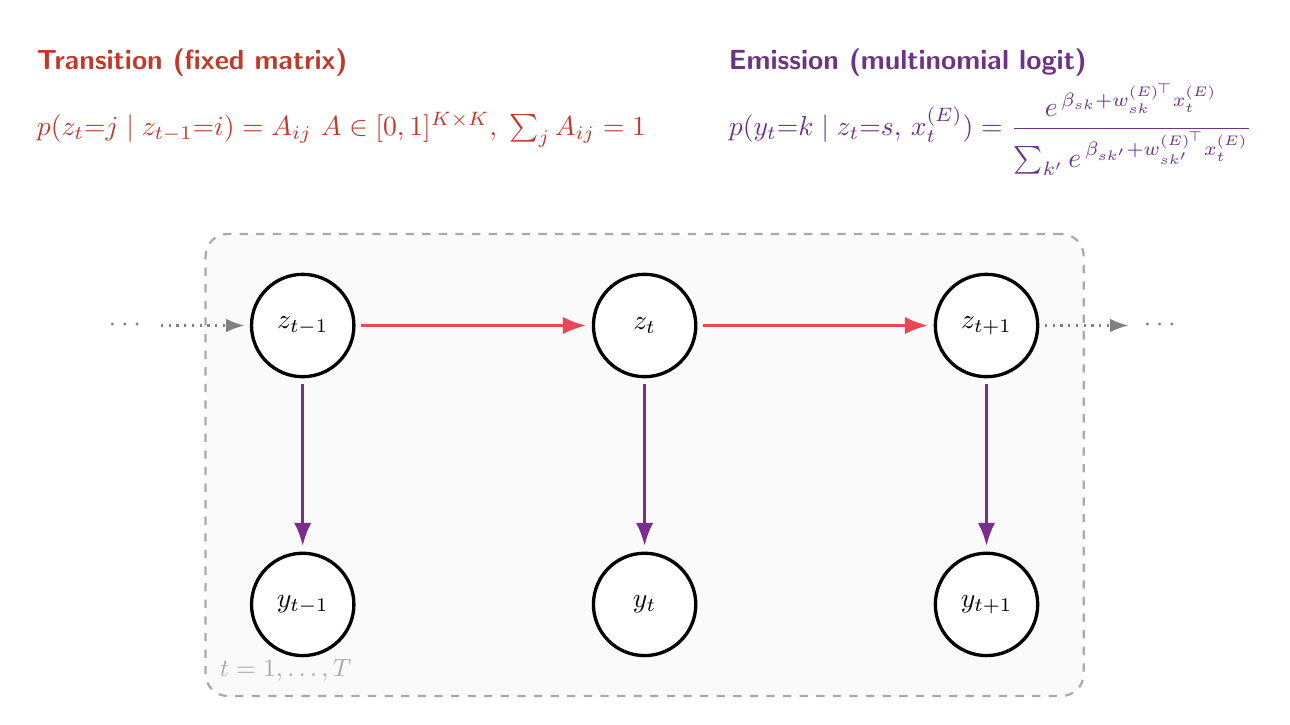
\begin{tikzpicture}[
  font=\sffamily,
  >=Latex,
  %% Node styles
  state/.style={
    circle, draw=black, fill=white,
    very thick, minimum size=13mm, inner sep=0pt,
    font=\sffamily\bfseries
  },
  obs/.style={
    circle, draw=black, fill=white,
    very thick, minimum size=13mm, inner sep=0pt,
    font=\sffamily\bfseries
  },
  %% Arrow styles
  tarrow/.style={->, very thick, color=transOrange,
                 shorten >=2pt, shorten <=2pt},
  earrow/.style={->, very thick, color=emitPurple,
                 shorten >=2pt, shorten <=2pt},
  dotarrow/.style={->, thick, dotted, color=black!50,
                   shorten >=2pt, shorten <=2pt},
]

%% ── Hidden states ──────────────────────────────────────────────────────────
\node[state] (z0) {$z_{t-1}$};
\node[state, right=30mm of z0] (z1) {$z_t$};
\node[state, right=30mm of z1] (z2) {$z_{t+1}$};

%% entry / exit dots
\node[left=12mm  of z0, text=black!50] (ldots) {$\cdots$};
\node[right=12mm of z2, text=black!50] (rdots) {$\cdots$};

%% ── Observations ───────────────────────────────────────────────────────────
\node[obs, below=22mm of z0] (y0) {$y_{t-1}$};
\node[obs, below=22mm of z1] (y1) {$y_t$};
\node[obs, below=22mm of z2] (y2) {$y_{t+1}$};

%% ── Transition arrows ──────────────────────────────────────────────────────
\draw[dotarrow] (ldots) -- (z0);
\draw[tarrow]   (z0)    -- (z1);
\draw[tarrow]   (z1)    -- (z2);
\draw[dotarrow] (z2)    -- (rdots);

%% ── Emission arrows ────────────────────────────────────────────────────────
\draw[earrow] (z0) -- (y0);
\draw[earrow] (z1) -- (y1);
\draw[earrow] (z2) -- (y2);

%% ── Plate ──────────────────────────────────────────────────────────────────
\begin{scope}[on background layer]
  \node[
    rounded corners=8pt,
    draw=plateGray, thick, dashed,
    fill=gray!4,
    inner xsep=16pt, inner ysep=14pt,
    fit=(z0)(z1)(z2)(y0)(y1)(y2)
  ] (plate) {};
\end{scope}
\node[above right=2pt and 2pt of plate.south west,
      font=\sffamily\small, text=plateGray] {$t = 1, \dots, T$};

%% ── Annotations (aligned table, no lines) ─────────────────────────────────
\node[
  above=6mm of plate.north, anchor=south,
  font=\sffamily
] (annos) {%
  \renewcommand{\arraystretch}{1.4}%
  \begin{tabular}{@{}l@{\qquad\quad}l@{}}
    \color{annoTrans}\textbf{Transition (fixed matrix)}
      & \color{annoEmit}\textbf{Emission (multinomial logit)} \\
    \color{annoTrans}$p(z_t{=}j \mid z_{t-1}{=}i) = A_{ij}$     \color{annoTrans}$A \in [0,1]^{K\times K},\;\textstyle\sum_j A_{ij}=1$
      & \color{annoEmit}$\displaystyle p(y_t{=}k \mid z_t{=}s,\,x^{(E)}_t)
          = \frac{e^{\,\beta_{sk}+{w^{(E)}_{sk}}^{\!\top} x^{(E)}_t}}
                 {\sum_{k'}e^{\,\beta_{sk'}+{w^{(E)}_{sk'}}^{\!\top} x^{(E)}_t}}$ \\[4pt]
  \end{tabular}%
};


\end{tikzpicture}
\end{document}